\chapter{Benutzeranleitung}
\label{Benutzeranleitung}

\lstset{
	breaklines=true,
	frame=single,
	language=bash,
}

\section{Installationsvoraussetzungen}
Zum Ausführen des Programms muss die Java Runtime Environment der Version 1.8.0\_121 oder eine höhere Version installiert sein. Ein Java Development Kit (JDK) mit gleichen Versionsanforderungen ist zusätzlich notwendig, wenn das Softwaresystem auch kompiliert werden soll.
Die zur Verfügungen gestellten Skripte sind Python-Skripte, um diese ausführen zu können wird Python Version 3.4 oder höher benötigt.
Unter Windows kann Git Bash (Git Version 2.10.2) als Shell verwendet werden.
Alle zur Verfügung gestellten Skripte wurden unter Windows mit Git Bash getestet und sind dort lauffähig. Sie wurden nicht auf anderen Systemen getestet.

\section{Installation}
Das gesamte Softwaresystem wird in Form einer zip-Datei bereitgestellt. Diese Datei muss entweder in das Verzeichnis, in dem das Programm installiert werden soll, kopiert und dort entpackt werden, wobei das Entpacken durch die Eingabe des folgenden Befehls erfolgt:

\begin{lstlisting}
	unzip grebing.zip
\end{lstlisting}

Oder die Datei kann mit Angabe des Verzeichnisses entpackt werden ohne, dass sie vorher im richtigen Verzeichnis liegen muss, dies ist möglich durch folgende Befehlseingabe:

\begin{lstlisting}
	unzip grebing.zip -d <Zielverzeichnis>
\end{lstlisting}

In Abbildung \ref{grafik:verzeichnisstruktur} ist die Verzeichnisstruktur des Installationsordner zu sehen. Im Ordner \textit{dist} ist die ausführbare \textit{gropro_2017_grebing.jar}-Datei zu finden, welche das Programm ausführt. Der Ordner \textit{bin} befinden sich alle kompilierten Java-Dateien in Form von \textit{.class}-Dateien. Der \textit{src}-Ordner enthält den gesamten Quellcode des erzeugten Softwaresystems. Im \textit{doc}-Ordner ist die \textit{javadoc}-Dokumentation in Form von \textit{.html}-Dateien zu finden. Die Datei \textit{index.html} ist der Einstiegspunkt in die \textit{javadoc}-Dokumentation. Der Ordner \textit{tests} enthält die Eingabedateien aller Testfälle und auch die Ausgabedateien von Normal- und Sonderfällen, nicht aber von Fehlerfällen, da diese keine Ausgabedatei erzeugen. Dabei haben Eingabedateien die Endung \textit{.in} und Ausgabedateien die Endung \textit{.out}.

\begin{figure}[H]
	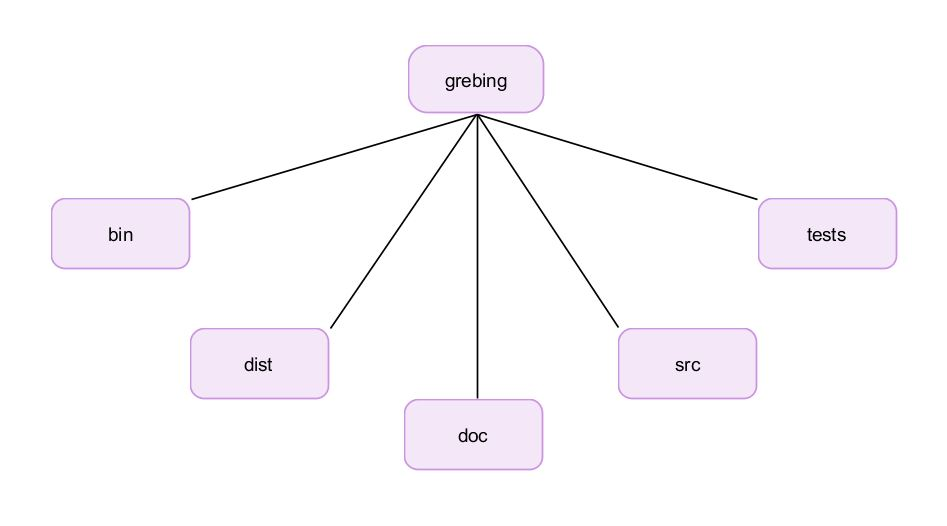
\includegraphics[width=15cm]{./Graphics/verzeichnisstruktur.JPG}
	\caption{Verzeichnisstruktur des Installationsordners}
	\label{grafik:verzeichnisstruktur}
\end{figure}



\section{Kompilieren des Programms}
Im folgenden wird vorausgesetzt, dass man sich im Installationsverzeichnis \textit{grebing} befindet.
Das Programm kann mit dem installierten Java-Kompiler kompiliert werden, indem der folgende Befehl verwendet wird:

\begin{lstlisting}
	javac src/*/*.java -d bin
\end{lstlisting}

\section{Ausführen des Programms}
Für den Aufruf des Programms ist es ebenfalls notwendig, das man sich im Installationsverzeichnis \textit{grebing} befindet. Dann kann das Programm mit folgendem Befehl ausgeführt werden:

\begin{lstlisting}
	java -jar dist/gropro_2017_grebing.jar <Eingabedatei> [<Ausgabedatei>]
\end{lstlisting}

Dem Programm müssen ein oder zwei Eingabeparameter übergeben werden. Dabei ist der erste Eingabeparameter der relative Pfad zur Eingabedatei und hat die Endung \textit{.in}. Der optionale zweite Eingabeparameter ist der relative Pfad zur Ausgabedatei und besitzt die Endung \textit{.out}. Sollte nur ein Eingabeparameter übergeben werden, so wird die Ausgabedatei im selben Ordner wie die Eingabedatei abgelegt.


\section{Ein- und Ausgabeformat}
Im Folgenden wird das zu verwendende Format der Eingabedatei sowie die Struktur der Ausgabedatei erläutert. Die genaue Beschreibung ist in den Abschnitten \ref{} und \ref{} zu enthalten.


\section{Mögliche Fehlermeldungen}




%Um die Tests automatisch auszuführen wird die bash-shell oder eine ähnliche benötigt.